\section{Introduction}
The goal is to measure the influence of Bluetooth Low Energy 
(BLE) on an existing WiFi network. Both wireless technologies 
use the same frequency of 2.4\,GHz. The work of 
\cite{Lansford.2001} measured the throughput of Wi-Fi in the 
presence of Bluetooth. \prettyref{fig:EvaluationWiFiBluetooth} 
shows to what extent the throughput is influenced with activated 
Bluetooth in 1\,m distance.

\begin{figure}
	\centering
	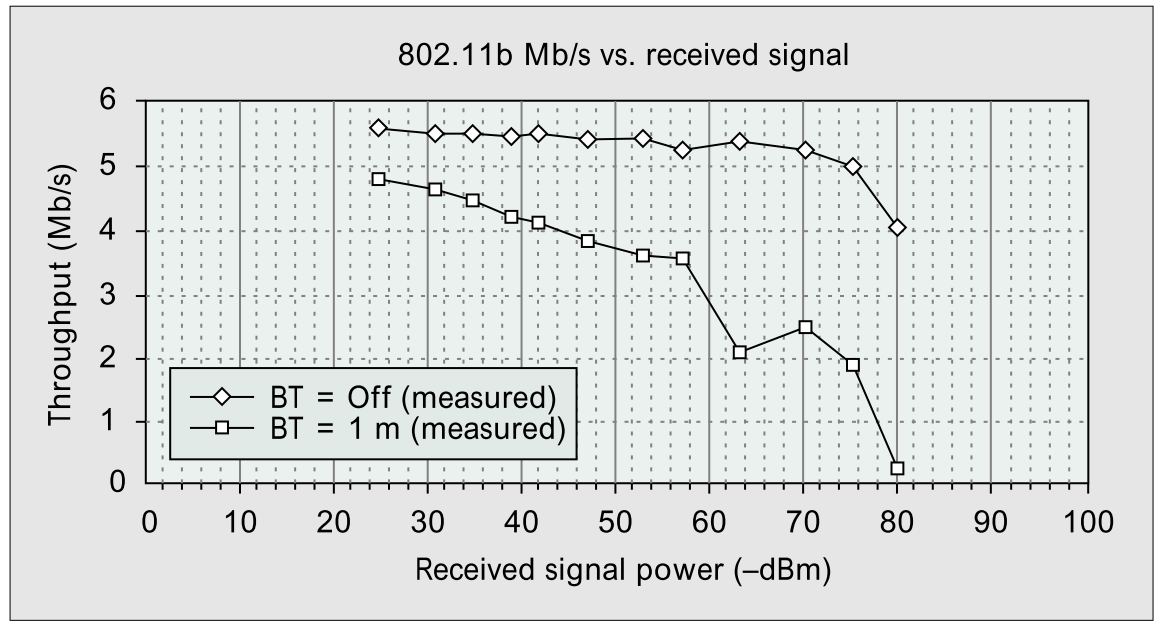
\includegraphics[width=0.4\textwidth]{evaluation_wifi_bluetooth}
	\caption{Measured throughput of Wi-Fi in the presence of 
	Bluetooth \cite{Lansford.2001}.}
	\label{fig:EvaluationWiFiBluetooth}
\end{figure}

A small delay of device discovery might occur depending on which 
WiFi channels are used, since BLE advertisers typically use 
three advertising channels randomly \cite{Wyffels.2014}. A more 
serious issue can be the decrease of the actual WiFi throughput. 
The paper \cite{Wyffels.2014} found two best practices. Randomly 
use available WiFi channels, if only low data rates have to be 
achieved. When high data rates need to be maintained, it is best 
to avoid WiFi channel 4 when a lot of BLE broadcasters are 
present. This choice ensures high WiFi throughput in presence of 
BLE devices.

\section{Testbed}
We established two different testbeds to measure the influence 
of BLE devices on a WiFi network. We use BLE beacons as BLE 
devices to enable indoor positioning and other proximity-based 
services. In both testbeds we simulate a worst case scenario by 
placing the BLE beacons around the access point to achieve a 
maximum disturbance.

The first testbed was installed at home in the basement without 
any discoverable WiFi network to measure only the influence of 
BLE beacons. The second testbed was installed at the university 
in a meeting room with many (approximately 110) nearby WiFi 
access points. \prettyref{fig:TestbedInstallation} shows the 
testbed installation. The distance between access point and 
client was 4\,m. \prettyref{tab:TestbedSettings} presents the 
difference between the two testbeds is the setting of the BLE 
beacons and and the test duration of the benchmark tool.

\begin{figure}
	\centering
	\small
	\begin{tabular}{cc}
		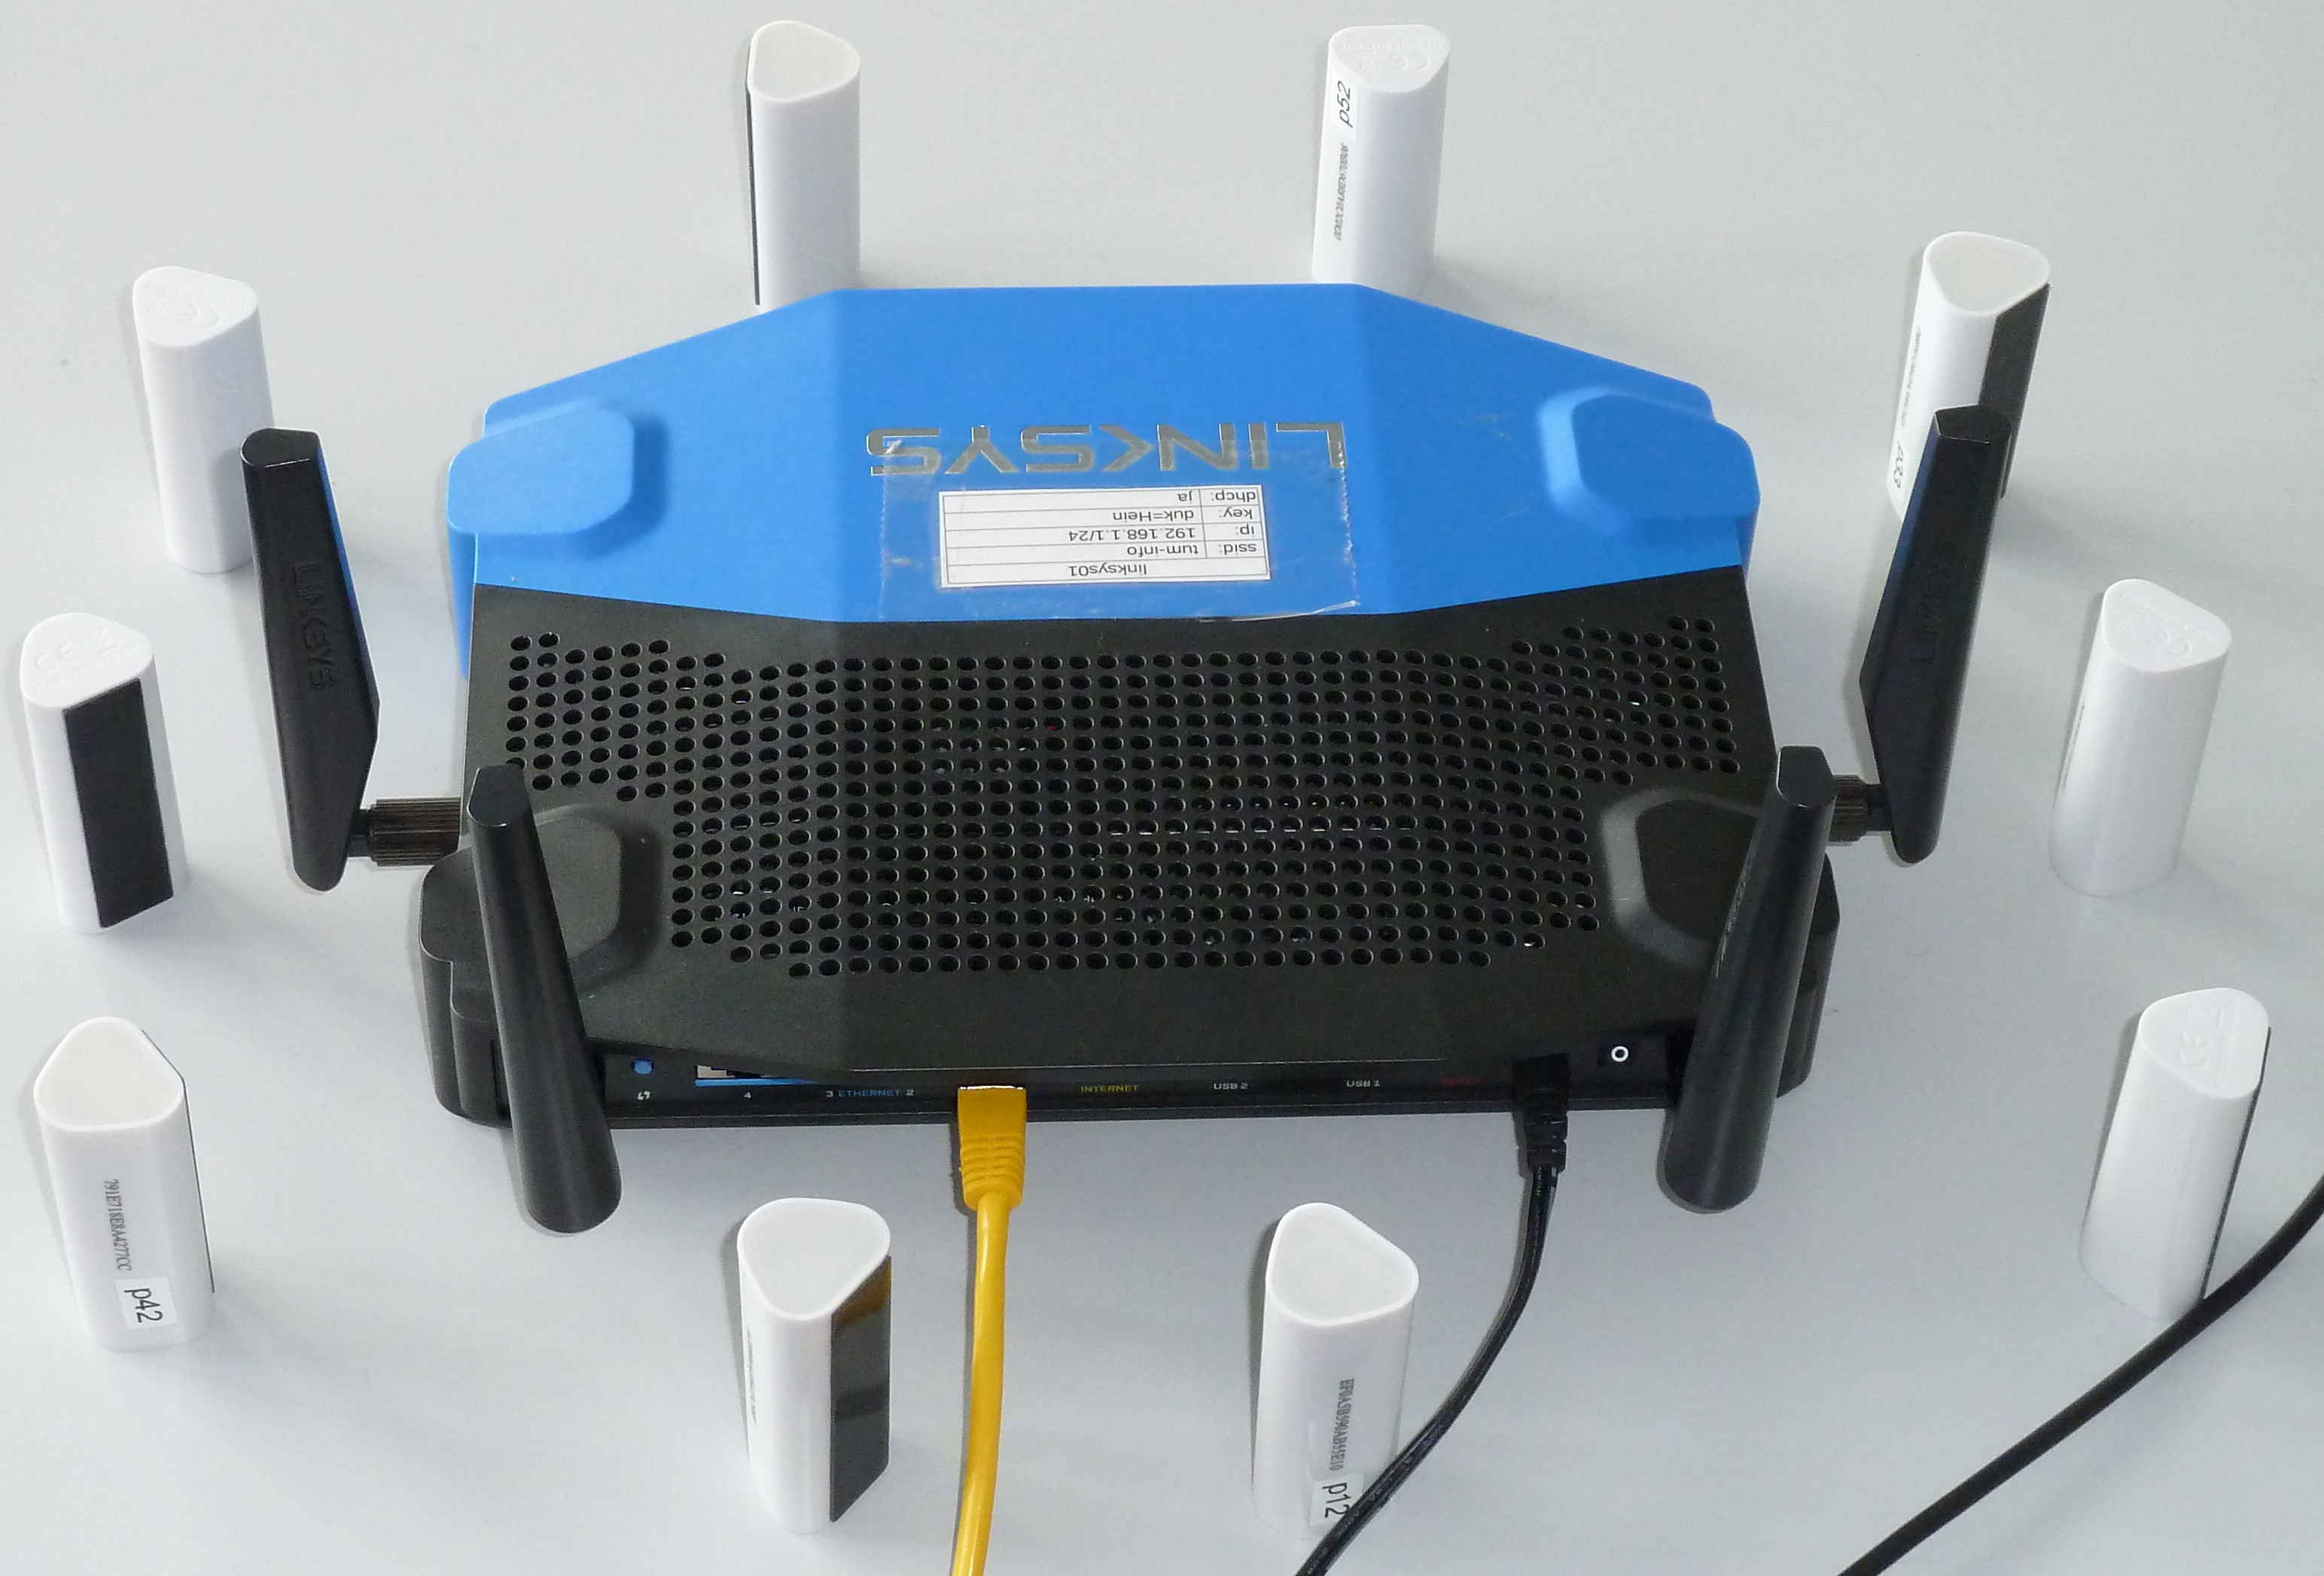
\includegraphics[width=0.2\textwidth]{testbed_router}
		&
		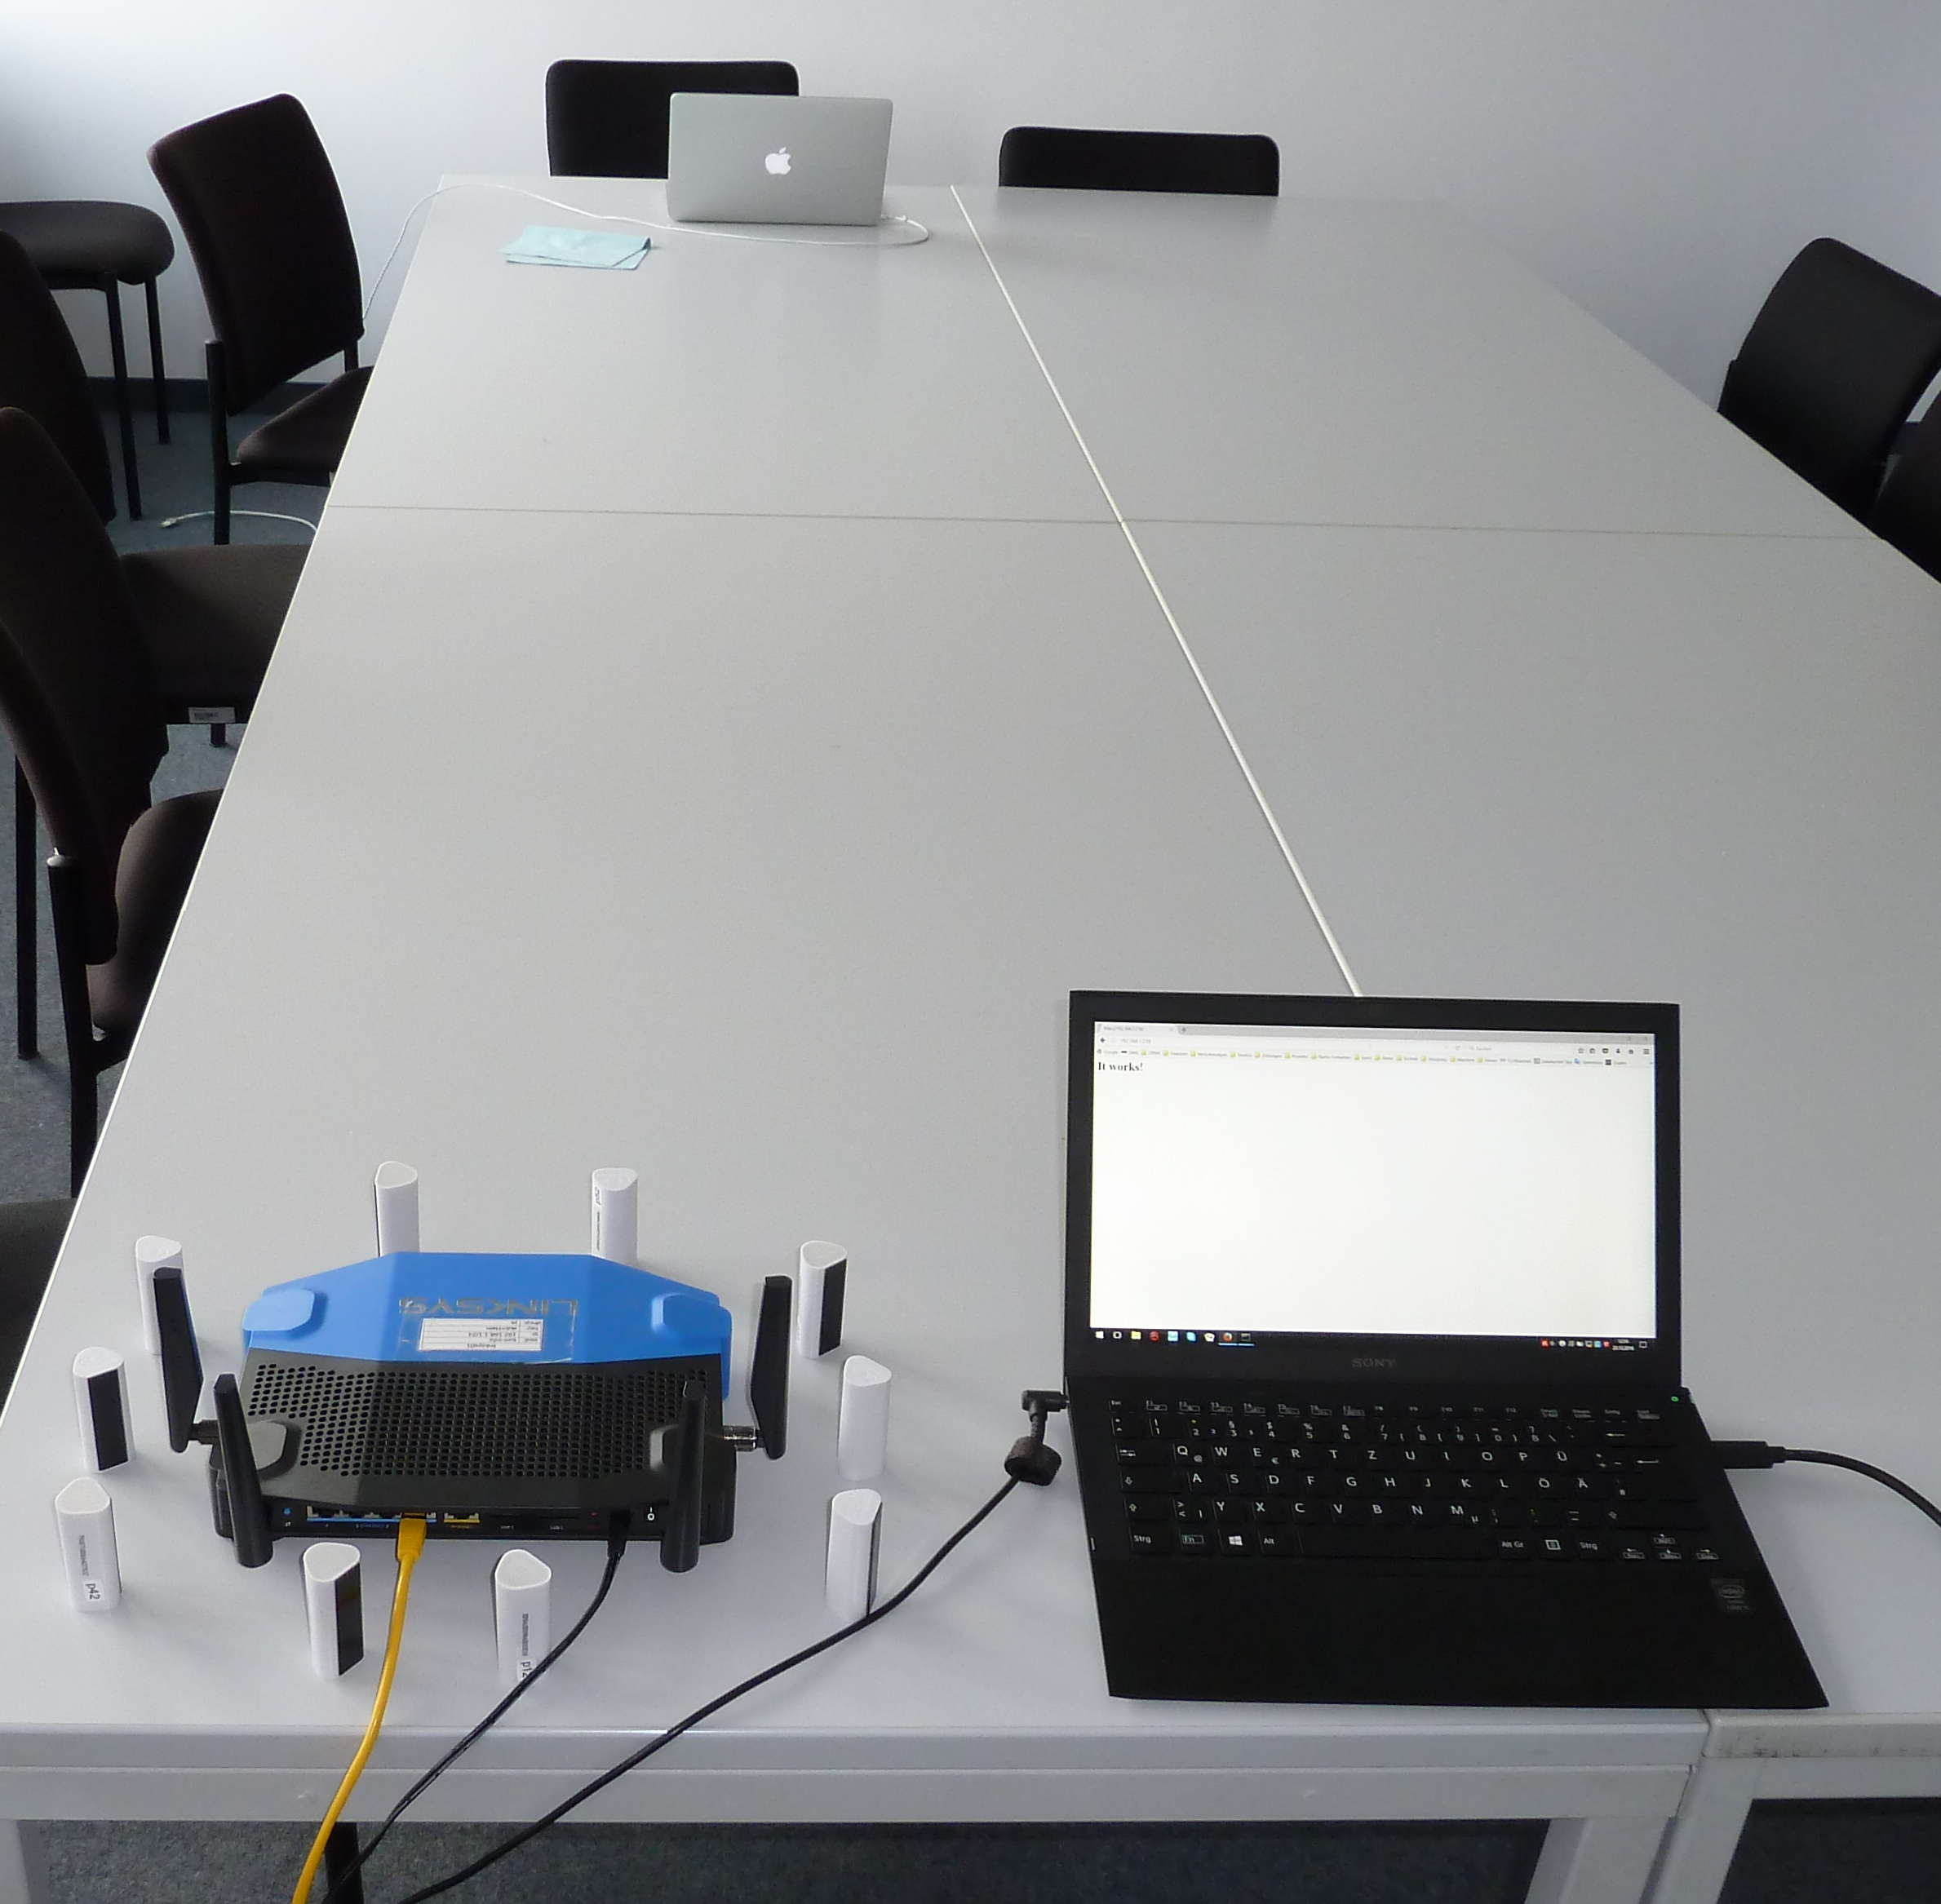
\includegraphics[width=0.2\textwidth]{testbed_setting}
		\\
		(a) Position of BLE beacons & (b) Testbed setting	
	\end{tabular}
	\caption{Testbed installation.}
	\label{fig:TestbedInstallation}
\end{figure}

\subsection{Hardware}
\begin{itemize}
	\item 1 x WiFi access point
	\begin{itemize}
		\item Linksys WRT 
		1900AC\footnote{\url{http://www.linksys.com/us/p/P-WRT1900AC/
		 (visited on 2016/12/27)}}
		\item SSID: tum-info
		\item Protocol: 802.11n
		\item Security: WPA2-Personal
		\item Network frequency: 2.4\,GHz
		\item Network channel: 1, 6
	\end{itemize}
	\item 1 x Apache Webserver (wired gigabit)
	\begin{itemize}
		\item Sony Vaio Pro 13
		\item CPU: Intel Core i5-4200U (1.6\,GHz)
		\item RAM: 8\,GB
	\end{itemize}
	\item 1 x Client (wireless)
	\begin{itemize}
		\item MacBook Pro Mid 2015
		\item CPU: Intel Core i5-5287U (2.9\,GHz)
		\item RAM: 16\,GB
		\item Network adapter: Broadcom 802.11ac
	\end{itemize}
	\item 10 x BLE beacons
	\begin{itemize}
		\item iBeek Sensor 
		Beacon\footnote{\url{http://bluvision.com/wp-content/uploads/2016/12/Specs-iBEEK1.6.pdf}
		 (visited on 2016/12/27)}
	\end{itemize}
\end{itemize}

\subsection{Software}
\begin{itemize}
	\item Apache Webserver 
	2.4.23\footnote{\url{http://www.apachelounge.com/} (visited 
	on 2016/12/27)}
	\item wrk benchmark 
	tool\footnote{\url{https://github.com/wg/wrk} (visited on 
	2016/12/27)}
\end{itemize}

\subsection{Testbed Setting}
\prettyref{fig:TestbedArchitecture} presents the general testbed 
consisting of a server client architecture. The Apache web 
server is connected via cable to the WiFi access and offers six 
dummy files: 1\,MB, 10\,MB, 50\,MB, 100\,MB, 500\,MB and 1\,GB 
which are used for the benchmark. The client uses a 2.4 GHz 
wireless connection to the access point and runs the wrk 
benchmark tool which uses the six dummy files from the Apache 
web server to measure the performance of the wireless 
connection. \prettyref{lst:BenchmarkScript} shows the wrk 
benchmark script. We have in total ten rounds for each of the 
six dummy files and calculate the average performance.

\begin{figure}
	\centering
	\begin{tikzpicture}	
	\tikzstyle{node} = [rectangle, text width = 2.3cm, very 
	thick, draw=black, align=center, inner sep=.5em, minimum 
	size=2em, text centered]
	\tikzstyle{arrow} = [draw, <->, >=latex, very thick]
	
	\node[node] (n1) {WiFi Access Point};	
	\node[node, below right=0.3cm of n1] (n2) {Apache Webserver};
	\node[node, below left=0.3cm of n1] (n3) {Client with wrk 
	benchmark tool};
	
	\path[arrow] (n1.east) -| node[above]{Wired} (n2);
	\path[arrow] (n1.west) -| node[align=left,above]{Wireless \\ 
	2.4 Ghz} (n3);
	\end{tikzpicture}
	\caption{Testbed with WiFi access point using only 2.4 GHz 
		wireless connection.}
	\label{fig:TestbedArchitecture}
\end{figure}

\begin{listing}
	\inputminted
	[
	frame=lines,
	framesep=2mm,
	breaklines,
	baselinestretch=1.2,
	fontsize=\footnotesize,
	]
	{bash}{"../wrk_performance.sh"}
	\caption{Benchmark script}
	\label{lst:BenchmarkScript}
\end{listing}

\prettyref{tab:TestbedSettings} shows all relevant testbed 
settings. The advertisement rate and range of the BLE beacons 
mainly influences the disturbance of the WiFi. These settings 
were used for beacon packets including S Beacon, Eddystone URL, 
Eddystone UID and Eddystone TLM (day and night mode). For the 
wrk benchmark tool we used only one thread and one connection. 
The test duration was firstly 30\,s in the worst case scenario 
and then extended to 60\,s in the real settings scenario. The 
reason was that the latency and requests are zero for bigger 
files ($\ge 50\,\text{MB}$) because the benchmark tool wrk was 
not able to finish the tests in the specified test duration due 
to the larger file size.

\begin{table}
	\caption{Testbed settings}
	\label{tab:TestbedSettings}
	\centering
	\begin{tabular}{L{1.5cm}lllll}
		\toprule
		& \multicolumn{2}{c}{Beacons} & 
		\multicolumn{3}{c}{Benchmark} \\		
		\cmidrule(r{2pt}){2-3}
		\cmidrule(l{2pt}){4-6}
		Testbed & Adv. rate & Range & Threads & Conn. & Duration 
		\\
		\midrule
		Worst case (home) & 0.1\,s & 80\,m & 1 & 1 & 
		30\,s \\
		\midrule
		Realistic settings (university) & 2.5\,s & 12\,m & 
		1 & 1 & 60\,s \\
		\bottomrule	
	\end{tabular}
\end{table}

\section{Evaluation Results}
The evaluation of the transfer size reflects best how the BLE 
beacons influence the WiFi performance. 
\prettyref{fig:EvaluationResultsTransferSize} shows that the 
transfer size is smaller in the presence of the BLE beacons. The 
testbed with realistic settings\footnote{less advertised 
beacon packets and smaller range} has smaller negative impact 
on the WiFi performance. However, the scenario with realistic 
beacon settings is still a worst case regarding the beacon 
placement, because the WiFi access point is surrounded by ten 
beacons in very short distance (few centimeters) which does not 
reflect the real testbed setting, in which the beacons have a 
distance of some meters. Thus, the effect of the BLE beacons is 
smaller.

\begin{figure}
	\centering
	\small
	\begin{tabular}{cc}
		\includegraphics[width=0.23\textwidth]{result/at_home/transfer}
		 &
		\includegraphics[width=0.23\textwidth]{result/at_university/transfer}
		\\
		(a) Worst case & (b) Realistic settings
		\\
		\multicolumn{2}{c}{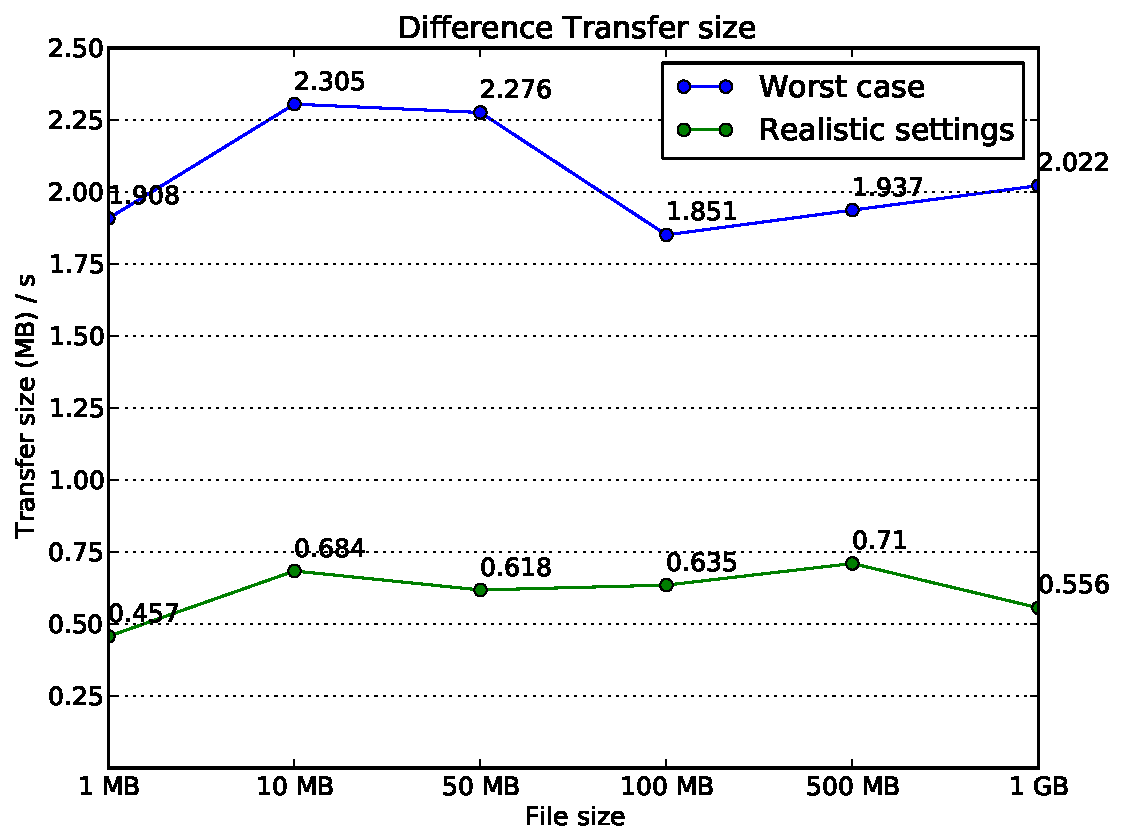
\includegraphics[width=0.23\textwidth]{result/difference_transfer_size}}
		\\		
		\multicolumn{2}{c}{Transfer size in presence of BLE 
		beacons and without BLE beacons.}
	\end{tabular}
	\caption{Evaluation results: Transfer size.}
	\label{fig:EvaluationResultsTransferSize}
\end{figure}

\prettyref{tab:EvaluationResultsTransferSize} shows the transfer 
size for the six dummy files in the two different testbeds. In 
the worst case scenario the transfer size is decreased by 1.91 
to 2.30\,MB/s (average: 2.05\,MB/s) and in the realistic setting 
scenario by 0.46 to 0.71\,MB/s (average: 0.61\,MB/s). These 
results show that the amount of advertised beacon packets and 
transmission strength (range) have a major impact on the WiFi 
performance. The ratio between the worst case and realistic 
settings is 3.36 regarding the transferred data.

\begin{table}
	\caption{Evaluation results: Transfer size}
	\label{tab:EvaluationResultsTransferSize}
	\centering
	\begin{tabular}{L{0.9cm}lllllll}		
		\toprule		
		& & \multicolumn{6}{c}{File size} \\	
		\cmidrule{3-8}
		Testbed & Setting & 1\,M & 10\,M & 50\,M & 
		100\,M & 500\,M & 1\,G \\
		\midrule
		\multicolumn{8}{c}{Transfer size (MB) / s} \\
		\midrule
		\multirow{4}{*}{\parbox{0.9cm}{Worst case}} & -\,BLE & 
		16.03 & 17.39 & 17.53 & 16.76 & 16.75 & 16.85 \\
		& +\,BLE & 14.12 & 15.09 & 15.25 & 14.91 & 14.82 & 14.82 
		\\
		\cmidrule{2-8}
		& Abs. & \textbf{1.91} & \textbf{2.30} & \textbf{2.28} & 
		\textbf{1.85} & \textbf{1.94} & \textbf{2.02} \\
		& Rel. & 11.90 & 13.25 & 12.98 & 11.04 & 11.56 & 12.00 \\
		\midrule
		\multirow{4}{*}{\parbox{0.9cm}{Realistic settings}} & 
		-\,BLE 
		& 9.69 & 10.42 & 10.44 & 10.34 & 10.24 & 10.18 \\
		& +\,BLE & 9.23 & 9.73 & 9.82 & 9.71 & 9.53 & 9.63 
		\\
		\cmidrule{2-8}
		& Abs. & \textbf{0.46} & \textbf{0.68} & \textbf{0.62} & 
		\textbf{0.64} & \textbf{0.71} & \textbf{0.56} \\
		& Rel. & 4.72 & 6.57 & 5.92 & 6.14 & 6.94 & 5.46 \\	
		\bottomrule
	\end{tabular}
\end{table}
